\documentclass[conference, 10pt]{IEEEtran}

\usepackage[utf8]{inputenc}
\usepackage[T1]{fontenc}
\usepackage{amsmath,amssymb}
\usepackage{graphicx}
\usepackage{booktabs}
\usepackage{multirow}
\usepackage{url}
\usepackage{hyperref}
\usepackage{xcolor}
\usepackage{balance}
\usepackage{enumitem}
\setlist{noitemsep,topsep=2pt}

\setlength{\textfloatsep}{4pt plus 1pt minus 1pt}
\setlength{\floatsep}{3pt plus 1pt minus 1pt}
\setlength{\intextsep}{3pt plus 1pt minus 1pt}
\setlength{\dbltextfloatsep}{4pt plus 1pt minus 1pt}
\setlength{\dblfloatsep}{3pt plus 1pt minus 1pt}

\hypersetup{
    colorlinks=true,
    linkcolor=blue!60!black,
    citecolor=blue!60!black,
    urlcolor=blue!60!black
}

\graphicspath{{../results/figures/}}

\title{Agreement Without Faithfulness:\\Do Consistent XAI Methods Produce Better Explanations?}

\author{
\IEEEauthorblockN{Angat Shah}
\IEEEauthorblockA{
Asha M. Tarsadia Institute of Computer Science and Technology (AMTICS)\\
Uka Tarsadia University\\
Bardoli, Gujarat, India\\
Email: angatshah1411@gmail.com}
}

\begin{document}

\maketitle

\begin{abstract}
Practitioners of Explainable AI (XAI) often validate explanations by comparing multiple methods: if SHAP and LIME agree, the explanation is assumed to be trustworthy. We empirically investigate whether this inter-method agreement is a reliable indicator of explanation quality. Using an XGBoost classifier on the UCI Adult Income dataset, we generate per-instance explanations via TreeSHAP, LIME, and Permutation Sensitivity, then evaluate their pairwise agreement (Spearman $\rho$, Kendall $\tau$, top-$k$ overlap), faithfulness (comprehensiveness and sufficiency), and stability under input perturbation. Our results show that (1)~methods exhibit moderate, highly variable agreement ($\rho = 0.43$--$0.75$), (2)~comprehensiveness and sufficiency produce consistent aggregate rankings but diverge at the per-instance level, (3)~inter-method agreement showed negligible-to-small negative associations with faithfulness (Spearman $\rho = -0.133$ to $0.004$, including a significant negative correlation between LIME and Permutation Sensitivity, $p = 0.003$), and (4)~SHAP and LIME show comparable stability despite different algorithmic foundations. These findings challenge the common heuristic that agreement implies quality, reinforcing LATEC's warning that XAI evaluation metrics can produce misleading conclusions.
\end{abstract}

\begin{IEEEkeywords}
Explainable AI, SHAP, LIME, feature attribution, faithfulness, explanation agreement, evaluation metrics, tabular data
\end{IEEEkeywords}

% ============================================================================
\section{Introduction}
\label{sec:introduction}
% ============================================================================

As machine learning models are deployed in high-stakes domains---credit scoring, healthcare, criminal justice---the demand for interpretable predictions has driven rapid growth in Explainable AI (XAI)~\cite{guidotti2018survey, molnar2020interpretable}. Among the most widely adopted methods are SHAP (SHapley Additive exPlanations)~\cite{lundberg2017shap} and LIME (Local Interpretable Model-agnostic Explanations)~\cite{ribeiro2016lime}, both of which produce per-instance feature importance scores.

A common but largely unexamined practitioner heuristic is to treat agreement between explanation methods as evidence of quality: \emph{``If SHAP and LIME agree on the important features, the explanation must be right.''} This reasoning is intuitive but not theoretically justified. Different methods embed different assumptions about locality, linearity, feature independence, and the reference distribution; agreement between two such methods need not imply that either is faithful to the model's decision process.

Recent large-scale benchmarks have revealed that evaluation metrics for XAI can produce conflicting rankings of methods. In particular, LATEC~\cite{hedstrom2024latec} evaluated 17~XAI methods across 20~metrics, multiple model architectures, and diverse modalities (spanning 7,560 combinations), demonstrating that metric selection alone can invert conclusions about which method is ``best.'' Other studies have documented widespread disagreement among attribution methods across vision, NLP, and tabular models~\cite{krishna2022disagreement, zhou2022feature}.

However, the question of whether \emph{inter-method agreement itself} can serve as an informal proxy for explanation quality remains underexplored, particularly on tabular data---the dominant modality in industry applications. Tabular XAI evaluation faces distinctive challenges: feature masking can create out-of-distribution inputs~\cite{hooker2019benchmark}, categorical features cannot be meaningfully perturbed by gradient-based methods, and objective ground truth for feature importance is absent.

In this work, we present a compact, controlled empirical study on tabular data that directly tests whether inter-method agreement is informative about faithfulness. Our contributions are:

\begin{enumerate}[leftmargin=*]
    \item We measure per-instance agreement between three XAI methods (TreeSHAP, LIME, Permutation Sensitivity) on tabular data, documenting substantial variability.
    \item We evaluate whether different faithfulness metrics (comprehensiveness, sufficiency) agree on which method is best, both in aggregate and per-instance.
    \item We test whether higher inter-method agreement predicts higher faithfulness, finding that it does not.
    \item We compare explanation stability under semantically reasonable input perturbations and test LIME's internal random seed sensitivity.
\end{enumerate}

Our study is intentionally small and focused: one dataset, one model, three methods, two faithfulness metrics. This design prioritizes depth over breadth, allowing us to examine contradictions and failure cases rather than reporting only averages.

% ============================================================================
\section{Related Work}
\label{sec:related-work}
% ============================================================================

\paragraph{Feature Attribution Methods.}
SHAP~\cite{lundberg2017shap} unifies several attribution methods under the framework of Shapley values~\cite{shapley1953value}, providing theoretical guarantees of local accuracy, missingness, and consistency. For tree-based models, TreeSHAP~\cite{lundberg2020treeshap} computes exact Shapley values in polynomial time. LIME~\cite{ribeiro2016lime} constructs a local linear surrogate model by sampling perturbations around the instance of interest. Permutation Sensitivity~\cite{fisher2019permutation, breiman2001random} adapts feature permutation to measure local instance-level sensitivity via prediction change.

\paragraph{Explanation Disagreement.}
Krishna et al.~\cite{krishna2022disagreement} surveyed practitioners and found that explanation methods frequently disagree, creating confusion about which to trust. Zhou et al.~\cite{zhou2022feature} systematically documented disagreement among attribution methods and showed it persists across model types. These studies establish that disagreement is common but do not investigate whether agreement, when it occurs, is a useful signal.

\paragraph{Faithfulness Evaluation.}
Faithfulness---the degree to which an explanation accurately reflects the model's reasoning---is commonly evaluated through perturbation-based metrics. DeYoung et al.~\cite{deyoung2020eraser} introduced comprehensiveness and sufficiency for NLP; these have been adapted for tabular settings. Samek et al.~\cite{samek2017evaluating} proposed pixel-flipping for image explanations. Yeh et al.~\cite{yeh2019infidelity} defined infidelity and sensitivity as complementary faithfulness measures. Hooker et al.~\cite{hooker2019benchmark} warned that removing features from trained models can produce out-of-distribution inputs, making faithfulness scores unreliable---a concern especially relevant for tabular data.

\paragraph{Metric Disagreement.}
LATEC~\cite{hedstrom2024latec} provided the most comprehensive evidence that XAI metrics disagree: across 7,560~method-metric-architecture combinations, rankings were highly sensitive to metric choice. Bhatt et al.~\cite{bhatt2020evaluating} showed that aggregation choices further compound this problem. Our work complements LATEC by testing metric agreement in the tabular domain and adding the novel dimension of asking whether inter-method agreement is informative about faithfulness.

% ============================================================================
\section{Research Questions and Hypotheses}
\label{sec:research-questions}
% ============================================================================

We investigate four research questions:

\noindent\textbf{RQ1:} \emph{How strongly do different XAI methods agree about feature importance rankings?}

\noindent\textbf{H1:} SHAP and LIME will show moderate but variable agreement ($\rho \in [0.4, 0.7]$), with substantial per-instance variability.

\noindent\textbf{RQ2:} \emph{How consistently do different faithfulness metrics rank explanation quality?}

\noindent\textbf{H2:} Comprehensiveness and sufficiency will produce partially conflicting method rankings.

\noindent\textbf{RQ3:} \emph{Does agreement between explanation methods correspond to greater faithfulness?}

\noindent\textbf{H3:} Higher inter-method agreement will \emph{not} reliably predict higher faithfulness.

\noindent\textbf{RQ4:} \emph{How stable are explanations under small, semantically reasonable input perturbations?}

\noindent\textbf{H4:} TreeSHAP explanations will be more stable than LIME explanations due to LIME's stochastic sampling.

% ============================================================================
\section{Methodology}
\label{sec:methodology}
% ============================================================================

\subsection{Dataset}

We use the UCI Adult Income dataset~\cite{adult_dataset}, a binary classification task predicting whether an individual's annual income exceeds \$50K. After removing missing values, the dataset contains 45,222 instances with 14 features (6~continuous, 8~categorical). We split the data 80/20 stratified by class, yielding 36,177 training and 9,045 test instances.

\subsection{Model}

We train an XGBoost~\cite{chen2016xgboost} classifier with 300 estimators, max depth 6, learning rate 0.1, and subsample/colsample ratios of 0.8. Categorical features are ordinal-encoded. The model achieves 86.8\% accuracy, F1 = 0.712, and AUC = 0.925 on the test set, competitive with published benchmarks.

\subsection{XAI Methods}

We generate per-instance explanations using three methods:

\begin{itemize}[leftmargin=*]
    \item \textbf{TreeSHAP}~\cite{lundberg2020treeshap}: Exact Shapley values computed via the tree-path algorithm. TreeSHAP was computed on the model's default raw output scale; faithfulness was subsequently evaluated using predicted-class probabilities.
    \item \textbf{LIME}~\cite{ribeiro2016lime}: Local linear surrogate trained on 5,000 perturbation samples per instance. Inherently stochastic; we fix the random seed for reproducibility.
    \item \textbf{Permutation Sensitivity (PS)}: We construct a per-instance permutation-sensitivity measure by permuting each feature across the evaluation sample and measuring the absolute change in predicted probability for each instance. Averaged over 20 permutation repeats.
\end{itemize}

For agreement and faithfulness evaluation, we use the \emph{absolute} feature importance values (|SHAP values|, |LIME coefficients|, PS scores) to enable rank-based comparison.

\subsection{Agreement Metrics (RQ1)}

For each pair of methods, we compute per-instance:
\begin{itemize}[leftmargin=*]
    \item \textbf{Spearman $\rho$}: Rank correlation between feature importance vectors.
    \item \textbf{Kendall $\tau$}: Concordance-based rank correlation.
    \item \textbf{Top-$k$ overlap}: Jaccard-like proportion of shared features in the top-$k$ most important features ($k \in \{3, 5\}$).
\end{itemize}

\subsection{Faithfulness Metrics (RQ2)}

We evaluate faithfulness using comprehensiveness and sufficiency~\cite{deyoung2020eraser}:

\textbf{Comprehensiveness}: Remove the top-$k$ most important features (according to the explanation method) by replacing them with training-set median (continuous) or mode (categorical), and measure the drop in predicted probability for the originally predicted class:
\begin{equation}
    \text{Comp}(x, k) = f(x)_c - f(x_{\setminus \text{top-}k})_c
\end{equation}
Higher comprehensiveness indicates the explanation correctly identified important features.

\textbf{Sufficiency}: Keep \emph{only} the top-$k$ features and mask all others:
\begin{equation}
    \text{Suff}(x, k) = f(x)_c - f(x_{\text{only top-}k})_c
\end{equation}
Lower sufficiency indicates the top-$k$ features are sufficient to reproduce the prediction.

We use $k \in \{1, 3, 5\}$ and include a \textbf{random baseline} that assigns uniformly random importance scores. The masking strategy (training-set median/mode) mitigates out-of-distribution concerns~\cite{hooker2019benchmark}.

\subsection{Agreement vs.\ Faithfulness Analysis (RQ3)}

For each method pair, we compute the per-instance Spearman~$\rho$ between the two methods' importance vectors (\emph{agreement}) and the average comprehensiveness at $k=3$ of both methods (\emph{faithfulness}). We then test the correlation between agreement and faithfulness using Pearson and Spearman correlations, and compare the mean faithfulness of the high-agreement group (above-median agreement) versus the low-agreement group using a Mann-Whitney $U$ test.

\subsection{Stability Analysis (RQ4)}

We perturb continuous features with Gaussian noise ($\sigma = 0.01 \times \text{feature range}$), leaving categorical features unchanged to preserve semantic validity~\cite{alvarez2018robustness}. For each of 100 randomly selected instances, we generate 10 perturbed copies, compute SHAP and LIME explanations for each, and measure stability as the Spearman $\rho$ between original and perturbed importance rankings. We compare SHAP and LIME stability via a Wilcoxon signed-rank test.

\subsection{Evaluation Sample}

From the 9,045 test instances, we select $N = 500$ via stratified sampling across prediction confidence terciles and predicted class, ensuring representation of both easy and difficult instances.

% ============================================================================
\section{Experimental Setup}
\label{sec:setup}
% ============================================================================

All experiments are implemented in Python using scikit-learn, XGBoost, SHAP, and LIME libraries. Random seeds are fixed at 42 throughout. The complete pipeline runs in approximately 30 seconds on a consumer laptop. Source code and results are provided for full reproducibility.

% ============================================================================
\section{Results}
\label{sec:results}
% ============================================================================

\subsection{Model Performance}

\begin{table}[htbp]
\centering
\caption{XGBoost Model Performance on Adult Income Dataset}
\label{tab:model-performance}
\begin{tabular}{lc}
\toprule
\textbf{Metric} & \textbf{Value} \\
\midrule
Accuracy & 0.8676 \\
F1 Score & 0.7122 \\
Precision & 0.7719 \\
Recall & 0.6610 \\
Roc Auc & 0.9250 \\
\bottomrule
\end{tabular}
\end{table}

The XGBoost model achieves 86.8\% accuracy with an AUC of 0.925 (Table~\ref{tab:model-performance}). This performance establishes a well-fitted predictive basis for the subsequent controlled explanation comparison across the evaluation sample. The moderate recall (0.661) reflects the class imbalance in the dataset (75.2\% negative class).

\subsection{RQ1: Explanation Agreement}

\begin{table}[htbp]
\centering
\caption{Pairwise Explanation Agreement (Mean $\pm$ SD)}
\label{tab:agreement}
\begin{tabular}{lccc}
\toprule
\textbf{Metric} & \textbf{SHAP vs LIME} & \textbf{SHAP vs PS} & \textbf{LIME vs PS} \\
\midrule
Spearman $\rho$ & $0.574 \pm 0.155$ & $0.749 \pm 0.118$ & $0.431 \pm 0.228$ \\
Kendall $\tau$ & $0.418 \pm 0.129$ & $0.592 \pm 0.118$ & $0.318 \pm 0.176$ \\
Top-3 overlap & $0.357 \pm 0.224$ & $0.649 \pm 0.208$ & $0.404 \pm 0.243$ \\
Top-5 overlap & $0.604 \pm 0.153$ & $0.741 \pm 0.147$ & $0.585 \pm 0.169$ \\
\bottomrule
\end{tabular}
\end{table}

Table~\ref{tab:agreement} summarizes the pairwise agreement between explanation methods. Several patterns emerge:

\textbf{SHAP and Permutation Sensitivity show the strongest agreement} (Spearman $\rho = 0.749 \pm 0.118$), consistent with both methods measuring prediction sensitivity to feature changes, albeit through different mechanisms.

\textbf{SHAP and LIME show moderate agreement} ($\rho = 0.574 \pm 0.155$), supporting H1. The standard deviation is large, indicating that agreement varies substantially across instances.

\textbf{LIME and Permutation Sensitivity show the weakest agreement} ($\rho = 0.431 \pm 0.228$), with the highest variability. This is notable because both are model-agnostic perturbation methods.

\begin{figure}[t]
    \centering
    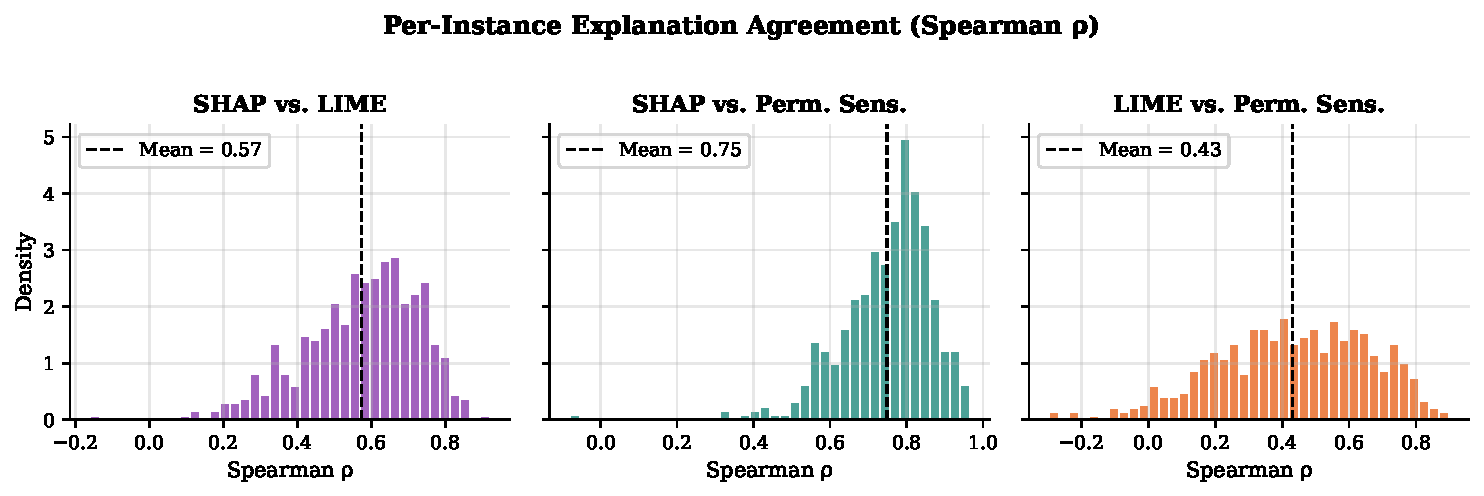
\includegraphics[width=0.92\columnwidth]{fig1_agreement_distributions.pdf}
    \caption{Distribution of per-instance Spearman $\rho$ between explanation methods. All distributions show substantial spread, with SHAP--LIME and LIME--PS exhibiting heavy left tails indicating frequent disagreement.}
    \label{fig:agreement-dist}
\end{figure}

Figure~\ref{fig:agreement-dist} reveals that the agreement distributions are not symmetric: all three pairs exhibit instances with near-zero or negative correlation, indicating complete disagreement on feature importance. The top-$k$ overlap analysis reinforces this finding: even at $k=5$ (covering 36\% of features), SHAP and LIME agree on only 60.4\% of top features.

\textbf{Finding (RQ1):} Methods agree moderately on average but disagree substantially for individual instances. Agreement cannot be assumed.

\subsection{RQ2: Faithfulness and Metric Agreement}

\begin{table*}[t]
\centering
\caption{Faithfulness Evaluation: Comprehensiveness and Sufficiency (Mean $\pm$ SD)}
\label{tab:faithfulness}
\begin{tabular}{llcccc}
\toprule
\textbf{Metric} & \textbf{$k$} & \textbf{SHAP} & \textbf{LIME} & \textbf{Perm.\ Sens.} & \textbf{Random} \\
\midrule
Comprehensiveness & $k=1$ & $0.1088 \pm 0.1654$ & $0.0268 \pm 0.1199$ & $0.0995 \pm 0.1676$ & $0.0087 \pm 0.0610$ \\
 & $k=3$ & $0.2269 \pm 0.1844$ & $0.0699 \pm 0.1549$ & $0.2042 \pm 0.2049$ & $0.0367 \pm 0.1019$ \\
 & $k=5$ & $0.3479 \pm 0.1942$ & $0.1346 \pm 0.1788$ & $0.3024 \pm 0.2136$ & $0.0742 \pm 0.1416$ \\
\midrule
Sufficiency & $k=1$ & $0.1518 \pm 0.1748$ & $0.3928 \pm 0.2180$ & $0.2554 \pm 0.2345$ & $0.3740 \pm 0.1941$ \\
 & $k=3$ & $0.0399 \pm 0.0939$ & $0.1810 \pm 0.1865$ & $0.0585 \pm 0.1074$ & $0.2780 \pm 0.2034$ \\
 & $k=5$ & $0.0138 \pm 0.0600$ & $0.1138 \pm 0.1474$ & $0.0166 \pm 0.0669$ & $0.1948 \pm 0.1893$ \\
\bottomrule
\end{tabular}
\end{table*}

Table~\ref{tab:faithfulness} presents comprehensiveness and sufficiency scores. SHAP consistently achieves the highest comprehensiveness and lowest sufficiency across all values of $k$. For comprehensiveness, methods rank consistently as SHAP $>$ PS $>$ LIME $>$ Random. For sufficiency, SHAP and PS outperform LIME and Random across all $k$; however, at $k=1$, Random outperforms LIME (sufficiency of $0.3740$ vs.\ $0.3928$), illustrating that at very small $k$, LIME's top feature is less sufficient than a randomly selected feature. The explanation methods generally outperform the random baseline under the evaluated faithfulness measures, although LIME does not outperform the random baseline on sufficiency at $k=1$.

\begin{figure}[t]
    \centering
    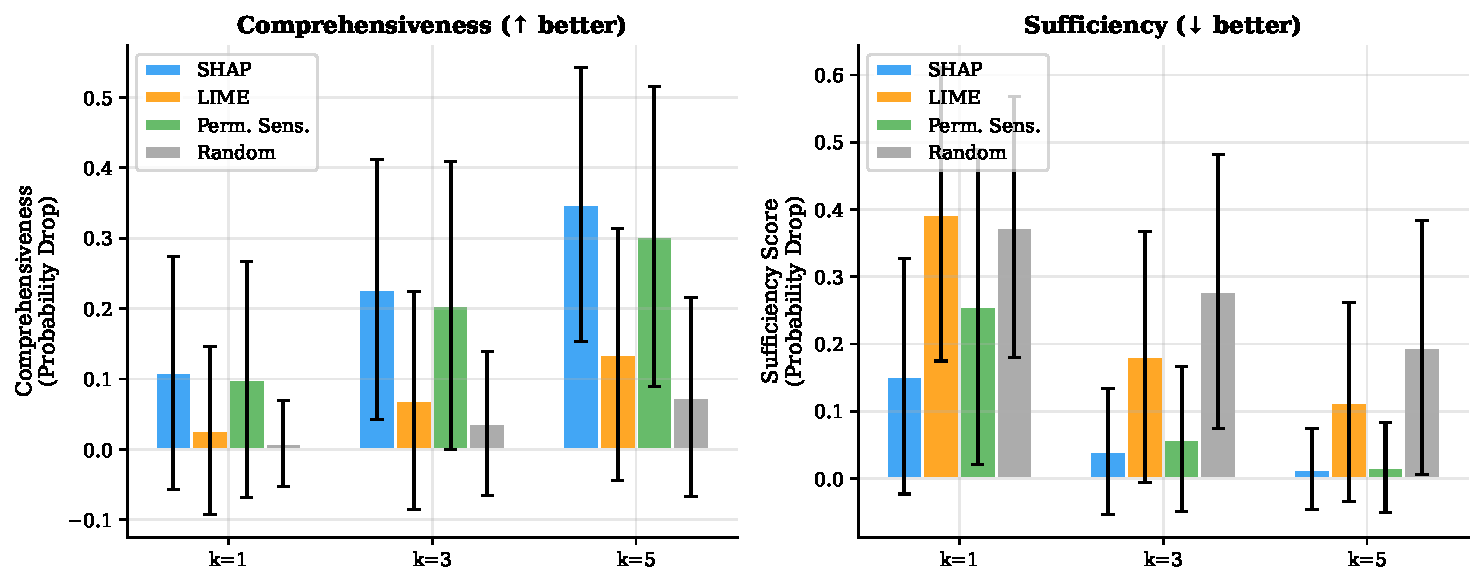
\includegraphics[width=0.92\columnwidth]{fig3_faithfulness.pdf}
    \caption{Comprehensiveness (left, higher is better) and sufficiency (right, lower is better) across methods and $k$ values. SHAP dominates on both metrics; LIME underperforms relative to Permutation Sensitivity.}
    \label{fig:faithfulness}
\end{figure}

\begin{figure}[t]
    \centering
    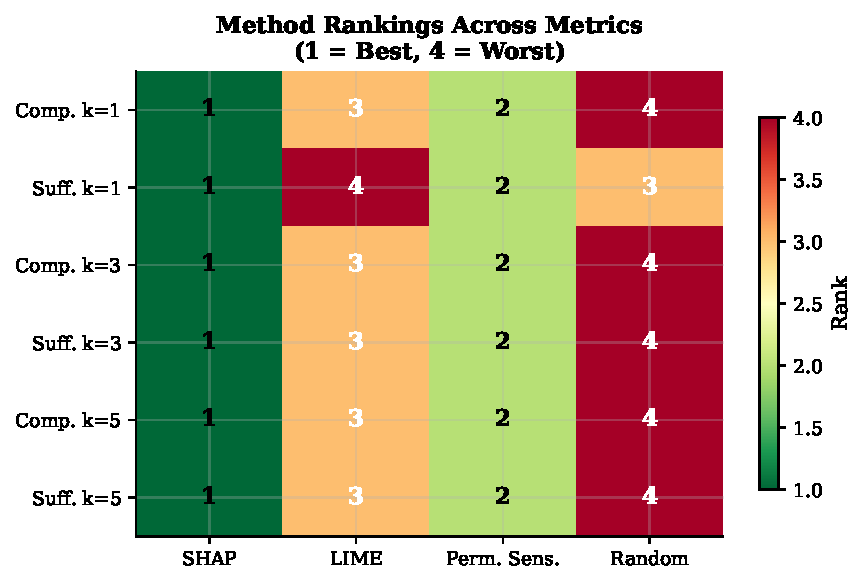
\includegraphics[width=0.92\columnwidth]{fig6_metric_rankings.pdf}
    \caption{Method rankings across faithfulness metrics and $k$ values. Rankings are largely consistent, with a notable exception at $k=1$ where sufficiency ranks Random above LIME.}
    \label{fig:rankings}
\end{figure}

\textbf{Aggregate metric agreement:} At $k \in \{3, 5\}$, comprehensiveness and sufficiency produce identical rankings (SHAP $>$ PS $>$ LIME $>$ Random). At $k=1$, sufficiency ranks Random above LIME (SHAP $>$ PS $>$ Random $>$ LIME), partially supporting H2.

\textbf{Per-instance metric agreement:} Although the aggregate rankings are stable, per-instance agreement between metrics is imperfect. The two metrics agree on the best method for a given instance 89.6\% of the time at $k=1$, dropping to 81.4\% at $k=5$. This means that for roughly 1 in 5--6 instances, comprehensiveness and sufficiency disagree about which method produced the best explanation.

\textbf{Finding (RQ2):} Comprehensiveness and sufficiency agree in aggregate but diverge for individual instances, supporting the concern that metric choice can affect conclusions, particularly at the instance level.

\subsection{RQ3: Agreement vs.\ Faithfulness}

\begin{table}[htbp]
\centering
\caption{Correlation Between Explanation Agreement and Faithfulness}
\label{tab:agree-vs-faith}
\resizebox{\columnwidth}{!}{%
\begin{tabular}{lccccc}
\toprule
\textbf{Method Pair} & \textbf{Spearman $r$} & \textbf{Raw $p$} & \textbf{Holm $p$} & \textbf{High Agree} & \textbf{Low Agree} \\
\midrule
SHAP vs LIME & $-0.083$ & $0.064$ & $0.129$ & $0.1403$ & $0.1566$ \\
SHAP vs PS & $0.004$ & $0.921$ & $0.921$ & $0.2140$ & $0.2170$ \\
LIME vs PS & $-0.133$ & $0.003$ & $0.009$ & $0.1380$ & $0.1361$ \\
\bottomrule
\end{tabular}%
}
\end{table}

\begin{figure}[t]
    \centering
    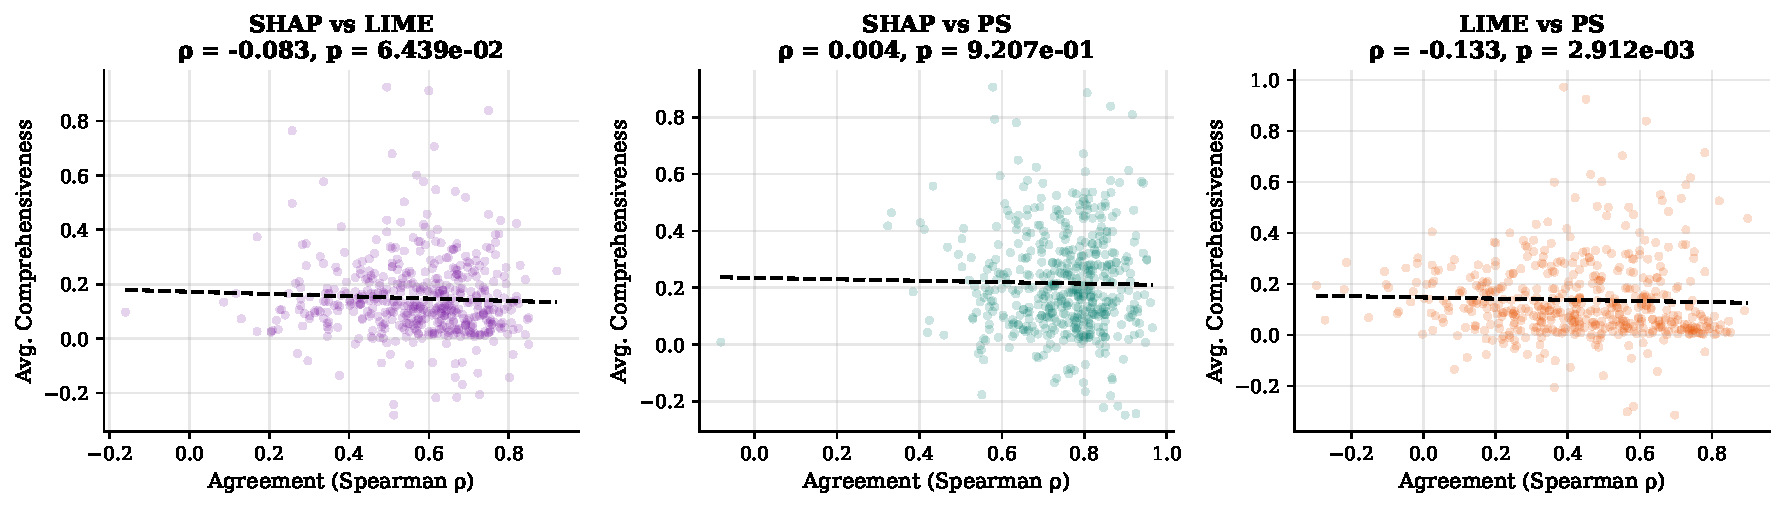
\includegraphics[width=0.92\columnwidth]{fig4_agreement_vs_faithfulness.pdf}
    \caption{Per-instance scatter of explanation agreement (Spearman $\rho$) vs.\ average comprehensiveness at $k=3$. No meaningful relationship is observed for any method pair.}
    \label{fig:agree-vs-faith}
\end{figure}

Table~\ref{tab:agree-vs-faith} and Figure~\ref{fig:agree-vs-faith} present the central result of this study. For all three method pairs, the correlation between inter-method agreement and pair-averaged faithfulness is negligible or negative: SHAP vs.\ LIME yields $r = -0.083$ (raw $p = 0.064$, Holm $p = 0.129$); SHAP vs.\ PS yields $r = 0.004$ (raw $p = 0.921$, Holm $p = 0.921$); and LIME vs.\ PS yields $r = -0.133$ (raw $p = 0.003$, Holm $p = 0.009$).

The LIME vs.\ PS pair shows a statistically significant but \emph{negative} correlation: instances where these methods agree more tend to have \emph{lower} faithfulness. After Holm correction for the three pairwise tests, this negative association remained statistically significant (adjusted $p = 0.009$). The Mann-Whitney $U$ tests comparing high- and low-agreement groups show no significant difference for any pair ($p > 0.07$).

\textbf{RQ3 Sensitivity Analysis:} To verify that these negligible and negative associations are not an artifact of evaluating pair-averaged faithfulness, we correlated inter-method agreement with each method's individual faithfulness score ($k=3$ comprehensiveness). For SHAP vs.\ LIME, agreement correlates with SHAP at $r = -0.141$ ($p = 0.002$) and with LIME at $r = 0.114$ ($p = 0.011$). For SHAP vs.\ PS, individual correlations remain near zero ($r = 0.024$, $p = 0.599$ for SHAP; $r = -0.001$, $p = 0.974$ for PS). For LIME vs.\ PS, agreement correlates positively with LIME ($r = 0.143$, $p = 0.001$) but negatively with PS ($r = -0.171$, $p < 0.001$). Across all pairs, correlations remain weak ($|r| \le 0.17$) and do not show joint positive alignment with the faithfulness of both methods, confirming that the central finding is not driven by pair-averaging.

\textbf{Finding (RQ3):} Under the studied experimental conditions, inter-method agreement was not a reliable positive predictor of explanation faithfulness. This directly challenges the common heuristic of using agreement as an informal quality check. H3 is supported.

\subsection{RQ4: Explanation Stability}

\begin{table}[htbp]
\centering
\caption{Explanation Stability Under Input Perturbation}
\label{tab:stability}
\begin{tabular}{lccc}
\toprule
\textbf{Method} & \textbf{Mean Stability ($\rho$)} & \textbf{Std} & \textbf{Median} \\
\midrule
SHAP & 0.876 & 0.062 & 0.895 \\
LIME & 0.886 & 0.046 & 0.894 \\
\midrule
\multicolumn{4}{l}{Wilcoxon $W = 2176$, $p = 0.297$ (rank-biserial $r = -0.121$)} \\
\bottomrule
\end{tabular}
\end{table}

\begin{figure}[t]
    \centering
    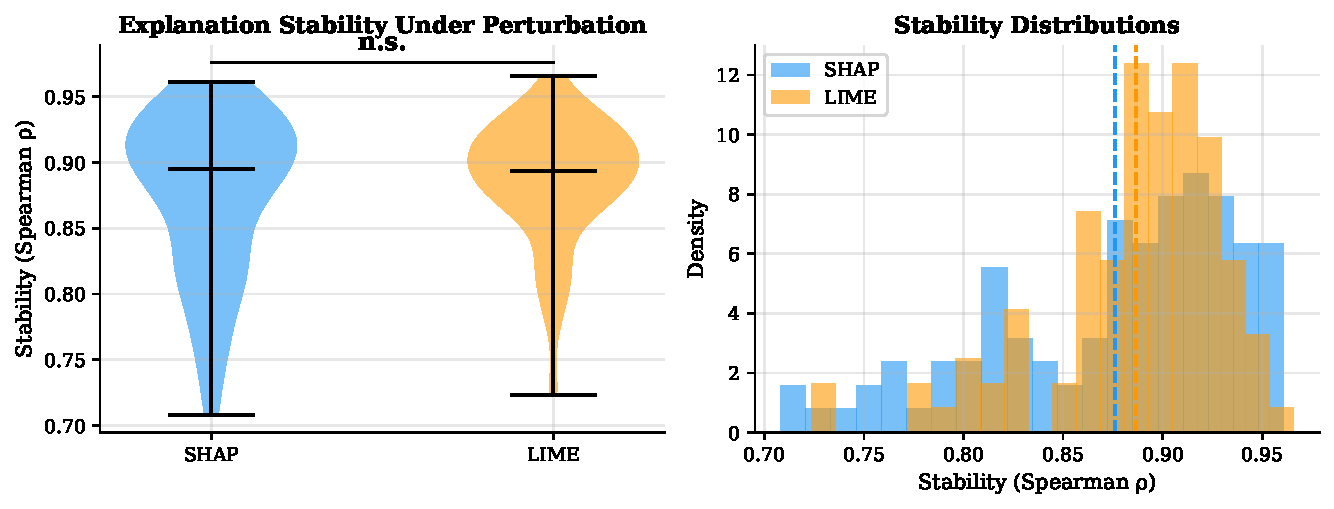
\includegraphics[width=0.92\columnwidth]{fig5_stability.pdf}
    \caption{Explanation stability under 1\% input perturbation. Both methods show high rank stability; the difference is not statistically significant.}
    \label{fig:stability}
\end{figure}

Both SHAP ($\rho = 0.876 \pm 0.062$) and LIME ($\rho = 0.886 \pm 0.046$) show high explanation stability under small continuous-feature perturbations (Table~\ref{tab:stability}, Figure~\ref{fig:stability}). The difference between methods is not statistically significant (Wilcoxon $W = 2176$, $p = 0.297$, matched-pairs rank-biserial $r = -0.121$).

\textbf{LIME Seed Sensitivity vs.\ Input Perturbation:} To distinguish input-perturbation stability from internal Monte Carlo sampling stochasticity, we held inputs fixed and computed LIME explanations across 10 independent random seeds on a 25-instance subset (5,000 perturbation samples each). Pairwise rank correlation across seeds showed high internal stability ($\rho = 0.925 \pm 0.014$, median $0.926$). This confirms that at 5,000 samples, LIME's internal sampling noise is minimal and that the observed high stability under 1\% input perturbation is not obscured by seed variability.

\textbf{Finding (RQ4):} Under the tested 1\% perturbation regime, both TreeSHAP and LIME produce stable feature rankings; LIME's internal sampling variance at 5,000 samples is similarly small. H4 is not supported in this local regime.

% ============================================================================
\section{Discussion}
\label{sec:discussion}
% ============================================================================

\paragraph{Agreement Is Not a Quality Signal}
The most important finding of this study is that inter-method agreement does not predict faithfulness (RQ3). This has direct practical implications: the common heuristic of ``if SHAP and LIME agree, the explanation is trustworthy'' is not supported by our evidence. Practitioners should not rely on agreement as a substitute for rigorous faithfulness evaluation.
The null result is an informative negative finding. If agreement were a valid quality indicator, we would expect at least a moderate positive correlation with comprehensiveness. Instead, correlations are negligible to slightly negative, indicating that agreement can even be a misleading signal.

\paragraph{Why Do Methods Agree When They Do?}
SHAP and Permutation Sensitivity show the strongest agreement ($\rho = 0.749$), likely because both fundamentally measure how predictions change when feature values are altered. SHAP does this via Shapley values (conditional expectations), while PS does it via sample permutation. LIME's weaker agreement with both methods reflects its distinct formulation: fitting a local linear model in a perturbed neighborhood.
The variability across instances is notable: some yield near-perfect agreement, others near-zero. Understanding the structural properties of instances with high vs.\ low agreement is a fruitful direction for future work.

\paragraph{SHAP's Faithfulness Advantage}
SHAP achieved the strongest faithfulness scores under the evaluation protocol used here. This result should not be interpreted as evidence that SHAP is universally more faithful, because the selected faithfulness metrics and intervention strategy may favor prediction-sensitivity approaches. TreeSHAP's performance reflects its exact Shapley computation, satisfying local accuracy, missingness, and consistency. LIME's lower faithfulness likely stems from surrogate approximation error. However, because the gap between SHAP and PS is smaller than between SHAP and LIME, measurement alignment is likely an influential factor: both attribution methods and faithfulness metrics evaluate prediction shifts under feature perturbation.

\paragraph{Metric Agreement: Aggregates vs.\ Instances}
Our finding that comprehensiveness and sufficiency agree in aggregate but diverge per-instance echoes LATEC's warning on a smaller scale. While aggregate rankings are stable, the metrics disagree on the best method for 10--19\% of individual instances, highlighting that metric selection directly impacts instance-level explanation deployment.

\paragraph{The Stability Surprise}
Contrary to our hypothesis, LIME was not less stable than TreeSHAP under 1\% input perturbation. Both methods exhibited high rank stability ($\rho \approx 0.88$). Coupled with our seed sensitivity analysis showing high internal Monte Carlo replicability ($\rho = 0.925$), this indicates that LIME's local sampling stochasticity does not translate into instability under the tested perturbation regime.

% ============================================================================
\section{Limitations and Threats to Validity}
\label{sec:limitations}
% ============================================================================

\begin{itemize}[leftmargin=*,itemsep=0.5pt,parsep=0pt,topsep=1pt]
    \item \textbf{Single dataset and model.} Findings are derived from the UCI Adult Income dataset and an XGBoost classifier; other datasets (medical, financial) and model families (e.g., neural networks) may display different agreement characteristics.
    \item \textbf{Categorical encoding.} Categorical variables were ordinal-encoded for cross-method compatibility; while suitable for controlled comparison, this introduces an artificial ordering that may affect tree split structure and attribution.
    \item \textbf{Masking strategy.} Feature replacement with training-set median/mode reduces out-of-distribution severity but does not guarantee joint-distribution realism~\cite{hooker2019benchmark}.
    \item \textbf{Metric circularity.} Comprehensiveness and sufficiency evaluate prediction sensitivity under feature removal, naturally favoring sensitivity-based attributions (SHAP, PS) over local linear surrogates (LIME).
    \item \textbf{LIME configuration.} LIME depends on hyperparameters (5,000 samples, exponential kernel width); alternate parameterizations may yield different fidelity characteristics.
    \item \textbf{Per-instance Permutation Sensitivity.} Our PS implementation measures per-instance prediction probability sensitivity under sample-wide permutation, differing from conventional global loss-based permutation importance.
    \item \textbf{No ground truth.} Ground truth feature importance is unavailable on real-world data; faithfulness scores serve as empirical proxies rather than direct correctness verifications.
    \item \textbf{Perturbation scale.} Stability analysis employed 1\% perturbations; larger perturbations may reveal latent instability outside the local neighborhood.
    \item \textbf{Absence of human evaluation.} Agreement, faithfulness, and stability are model-centric properties; we do not evaluate human plausibility or decision utility.
\end{itemize}

% ============================================================================
\section{Future Work}
\label{sec:future-work}
% ============================================================================

Several directions emerge from this study: (1)~\textbf{Multi-dataset validation} across diverse tabular domains; (2)~\textbf{Conditional instance analysis} examining when agreement correlates with faithfulness across confidence terciles; (3)~\textbf{Alternative faithfulness metrics} such as infidelity~\cite{yeh2019infidelity} and ROAR retraining~\cite{hooker2019benchmark}; (4)~\textbf{Human evaluation} assessing whether agreement correlates with human-perceived explanation utility; and (5)~\textbf{Neural tabular models} (e.g., TabNet) where gradient-based attributions apply.

% ============================================================================
\section{Conclusion}
\label{sec:conclusion}
% ============================================================================

We investigated whether agreement between XAI methods is a reliable indicator of explanation quality on tabular data. Through a controlled experiment with TreeSHAP, LIME, and Permutation Sensitivity on an XGBoost model trained on the UCI Adult Income dataset, we found that:
(1)~Methods agree moderately on average ($\rho = 0.43$--$0.75$) but exhibit large per-instance dispersion and occasional complete disagreement;
(2)~Comprehensiveness and sufficiency agree on aggregate method rankings (at $k \ge 3$) but diverge for 10--19\% of individual instances;
(3)~Under the studied experimental conditions, inter-method agreement was not a reliable positive predictor of faithfulness ($\rho = -0.133$ to $0.004$, confirmed by individual-method sensitivity analysis); and
(4)~Both SHAP and LIME demonstrate comparable stability under local input perturbation ($p = 0.297$), with LIME showing high internal seed stability ($\rho = 0.925$).

These findings challenge the common practitioner heuristic that agreement implies quality: two methods agreeing on feature importance provides no guarantee that either explanation faithfully reflects the model's reasoning. Practitioners should evaluate explanation quality through direct faithfulness metrics rather than relying on inter-method agreement. More broadly, our results reinforce the growing consensus~\cite{hedstrom2024latec, krishna2022disagreement} that XAI evaluation requires rigorous, multi-dimensional assessment rather than informal proxies.

% \balance
\section*{Reproducibility}

All source code, experimental configurations, raw results, and figure-generation scripts are provided with this manuscript. Experiments use fixed random seeds (seed = 42) and publicly available data. The complete pipeline runs in approximately 30 seconds on a consumer laptop.

\bibliographystyle{IEEEtran}
\bibliography{references}

\end{document}
